  Die Eignung, der zu evaluierenden Java Web Frameworks, wird durch eine Menge
  von Soll-Kriterien bestimmt. Die Soll-Kriterien bestimmen die Anforderungen,
  welche erfüllt werden sollen. Die Anforderungen stammen von einer
  Projektgruppe der Hochschule für Technik und Wirtschaft Berlin. Die
  Soll-Kriterien werden für den Einsatz in der \ac{ZKB} priorisiert.
  
  Soll-Kriterien sind Vorgaben, die möglichst weitgehend Erfüllt werden sollen.
  Wenn ein solches Kriterium nicht erfüllt werden kann, schliesst das die
  Alternative nicht aus. Jedem Soll-Kriterium wird für die Identifikation eine
  eindeutige ID vergeben. Die ID setzt sich folgendermassen zusammen: 
  \{Soll\}-\{Laufnummer\}.
  
  \section{Anforderungen an Web Frameworks nach AgileLearn}
  
  Eine Projektgruppe namens AgileLearn von der Hochschule für Technik und
  Wirtschaft Berlin befasst sich mit dem Thema Web Frameworks. Die
  Projektgruppe hat sich die Frage gestellt:
  
  \begin{quote}``\begin{itshape}Welche Anforderungen müssen bei der Wahl eines
  Webframeworks berücksichtigt werden?\end{itshape}'' \footnote{Zitat von Raoul
  Jaeckel, siehe \cite{AnforderungenAnWebframeworks}}
  \end{quote}
  
  Aus dieser Fragestellung heraus, wurden 18 Anforderungen an Web Frameworks
  ausgearbeitet, welche öffentlich in einem Google-Doc\footnote{Ein Service von
  Google um Dokumente öffentlich zu bearbeiten.} ersichtlich sind.
  
  Folgende Anforderungen stammen aus dem Dokument ``\begin{itshape}18
  Anforderungen an Webframeworks -
  OpenDoc\end{itshape}'', siehe \cite{AnforderungenAnWebframeworks}, und werden
  im Anhang \ref{chapter:18AnforderungenNachAgileLearn}
  \nameref{chapter:18AnforderungenNachAgileLearn} (auf Seite
  \pageref{chapter:18AnforderungenNachAgileLearn}ff) zusammengefasst und mit
  einer ID versehen.
    
  \section{Wichtige Aspekte im Software-Lebenszyklus für die Zürcher
  Kantonalbank}
  
  Die wichtigen Aspekte wurden in Absprache mit dem Auftraggeber ausgearbeitet.
  Es handelt sich dabei nur um sehr grundlegende Bedürfnisse der \ac{ZKB}:
  \newline
  
  \begin{description}
    \item[Sicherheit]
    Nur eine Bank, die als sicher gilt, hat das Vertrauen der Kunden und somit
    Erfolg in ihrem Geschäft.
    \item[Kosten]
    Die laufenden Kosten sollen so tief wie möglich gehalten werden. Gemäss
    Abbildung \ref{img:softwareLifecycleCost} liegen die Hauptkosten im
    Software-Lebenszyklus bei der Maintenance-Phase. Somit können die Kosten für
    requirements Engineering, Design, Programmierung und Integration
    vernachlässigt werden.
    \item[Ressourcen]
    Damit Software entwickelt und gewartet werden kann, wird die Verfügbarkeit
    von qualifizierten Ressourcen benötigt.
    \item[Image]
    Um sich von der Konkurrenz abzuheben wird ein Image aufgebaut das sich
    zeitgemäss, flexibel und innovativ präsentieren soll, siehe
    \cite{WillkommenBeiDerZkb} S. 34ff.
    \newline
  \end{description}
  
  \begin{figure}[ht]
    \begin{center}
      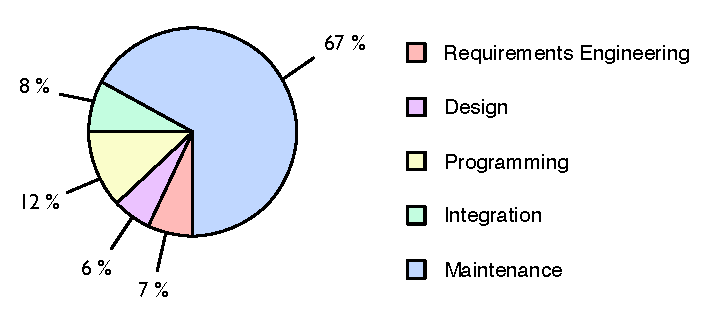
\includegraphics[width=0.9\textwidth]{./image/softwareLifeCycleCost.pdf}
      \caption{Ungefähre relative Kosten der Phasen des Software-Lebenszyklus
      (nach \cite{SoftwareEngineering} S. 11 und
      \cite{SoftwareLifeCycleModels})}
      \label{img:softwareLifecycleCost}
    \end{center}
  \end{figure}
  
  \clearpage
    
  \section{Priorisierung der Soll-Kriterien}
  
  Da 18 Soll-Kriterien definiert wurden und diese in jeder Alternative 
  untersucht werden müssten, würde das den Rahmen der Diplomarbeit sprengen.
  Deshalb sollen die Soll-Kriterien in eine Hierarchie entsprechend ihrer
  Wichtigkeit für die \ac{ZKB} aufgeteilt werden. Es sollen nur die
  ``wichtigen'' Soll-Kriterien in die Evaluation mit einbezogen werden. Die
  Hierarchie wird deshalb in drei Gruppen aufgeteilt:
  
  \begin{itemize}
    \item Wichtig
    \item Nice to have
    \item Unwichtig
  \end{itemize}
  
  \noindent
  Es soll eine Konsolidierung statt finden, zwischen den 18 Soll-Kriterien und
  den wichtigen Aspekten im Software-Lebenszyklus für die \ac{ZKB}. Die
  Konsolidierung wird in der Tabelle \ref{tab:kosolidierungDerSollKriterien}
  gezeigt. Die Soll-Kriterien mit zwei oder mehr + werden als ``wichtig'', mit
  einem + als ``nice to have'' und ohne + als ``nicht wichtig'' priorisiert. Die
  Gründe für die Priorisierung soll anschliessend erläutert werden.
  
  \begin{table}[htb]
    \sffamily 
    \begin{center}
      \begin{threeparttable}
        \begin{tabular}{p{9cm}cccc}
          \toprule
          \textbf{Anforderung} & \textbf{(Si)} & \textbf{(Ko)} & \textbf{(Re)} &
          \textbf{(Im)}\\
          \midrule
          \ref{itm:Soll-01} & ++ &    &    &    \\
          \ref{itm:Soll-02} & +  &    &    &    \\
          \ref{itm:Soll-03} &    & ++ &    &    \\
          \ref{itm:Soll-04} &    & +  &    &    \\
          \ref{itm:Soll-05} &    &    &    &    \\
          \ref{itm:Soll-06} & +  & ++ &    & ++ \\
          \ref{itm:Soll-07} &    &    &    &    \\
          \ref{itm:Soll-08} &    &    &    &    \\
          \ref{itm:Soll-09} &    &    &    &    \\
          \ref{itm:Soll-10} &    &    &    &    \\
          \ref{itm:Soll-11} &    &    &    &    \\
          \ref{itm:Soll-12} &    & ++ &    &    \\
          \ref{itm:Soll-13} &    &    & ++ &    \\
          \ref{itm:Soll-14} &    & +  &    &    \\
          \ref{itm:Soll-15} &    &    &    &    \\
          \ref{itm:Soll-16} &    &    &    &    \\
          \ref{itm:Soll-17} &    &    & +  &    \\
          \ref{itm:Soll-18} &    &    &    & ++ \\
          \bottomrule
        \end{tabular}
        \caption{Wie wichtig sind die Soll-Kriterien für die ZKB.}
        \label{tab:kosolidierungDerSollKriterien}
        \medskip 
        %\footnotesize\textbf{Legende:}\smallskip 
        \begin{tablenotes}[++]\footnotesize 
          \item[(Si)] Sicherheit 
          \item[(Ko)] Kosten in der Maintenance-Phase des Software-Lebenszyklus
          \item[(Re)] Ressourcen 
          \item[(Im)] Image
          \item[++] hat grossen Einfluss
          \item[+] hat Einfluss
        \end{tablenotes}
      \end{threeparttable}
    \end{center}
  \end{table}
  
  \subsection{Wichtig}
  
  Diese Soll-Kriterien dienen als Basis für den Kriterienkatalog, welcher in der
  gewichteten Nutzwertanalyse verwendet wird.
  
  Es handelt sich dabei hauptsächlich um grundlegende Anforderungen, die
  erfüllt werden müssen, damit Webapplikationen zeitgemäss entwickelt und
  später gewartet werden können.
  \newline
  
  \begin{description}
  \item[Soll-01 - Zugriffskontrolle]
  Auf die Sicherheit von Applikationen in einer Bank wird grossen Wert
  gelegt. Mit einer genügenden Authentifizierung, Autorisation und
  Rollenverwalung, kann eine Applikation sicher implementiert werden.
  
  \item[Soll-03 - Modulare Architektur]
  Um während der Maintenance-Phase des Software Lebenszyklus notwendige
  Anpassungen an einer Applikation machen zu können, ist eine modulare
  Architektur von grossem Vorteil. Zudem ist das auch während der
  Entwicklungs-Phase hilfreich.
  
  \item[Soll-06 - Testing]
  Um während der Maintenance-Phase des Software-Lebenszyklus notwendige
  Anpassungen an einer Applikation machen zu können, ist ein gutes Testing von
  grossem Vorteil. Das Testing hat auch einen grossen Einfluss auf das Image,
  denn wer möchte schon fehlerhafte Software verwenden. Durch eine gute
  Testbasis, kann auch die Sicherheit einer Applikation gesteigert werden.
  
  \item[Soll-12 - Dokumentation]
  Eine saubere und verständliche Dokumentation eines Web Application Frameworks
  ist das A und O, um während allen Software-Lebenszyklen effizient arbeiten zu
  können. Ein Web Application Framework mit einer tiefgreifenden Dokumentation
  hat bestimmt höhere Chancen sich längerfristig am Markt durchzusetzen.
  
  \item[Soll-13 - Community]
  Damit die notwendigen Ressourcen, für die Umsetzung und Wartung eines
  Software-Projekts gefunden werden, wird eine entsprechend grosse Community
  benötigt. Wenn die Community genügend gross ist, kann man davon ausgehen,
  dass auch in der Zukunft noch genügend Ressourcen in diesem Bereich
  erreichbar sind.
  
  \item[Soll-18 - AJAX-Unterstützung]
  In der Zeit von Google Mail, Facebook und Twitter wird die Verwendung von
  \ac{Ajax} unterstützten Web Applikationen zur Gewohnheit. Um mit einer Web
  Applikation ein zeitgemässes, flexibles und innovatives Image vermitteln zu
  können, sollten diese mit \ac{Ajax}-Unterstütztung gebaut werden.
  \end{description}
  
  \subsection{Nice to have}
  
  Diese Soll-Kriterien fliessen nicht in den Evaluationsprozess mit ein. Das
  Vorhandensein würde in der Entwicklungsphase aber sicher einen Erleichterung
  mit sich bringen.
  \newline
  
  \begin{description}
  \item[Soll-02 - Form-Validierung]
  Eine saubere Validierung der Formularfelder gehört zu den notwendigen
  Werkzeugen, um eine sichere Web Applikation zu entwickeln. Dennoch kann durch
  gutes Testing und eine sichere Zugriffskontrolle der selbe Effekt erzielt
  werden.
  
  \item[Soll-04 - Schnittstellen und Webservices]
  Durch die breite Unterstützung von Schnittstellen und Webservice Technologien
  in der Java Welt, muss ein Web Framework dies nicht schon von Haus aus
  mitbringen. Fall es doch vorhanden ist, um so besser.
  
  \item[Soll-14 - IDE-Unterstützung]
  Eine IDE-Unterstützung ist zu präferieren, soll aber kein Hindernis für den
  Einsatz eines guten Web Frameworks sein.
  
  \item[Soll-17 - Lernkurve für EntwicklerInnen]
  Durch die Unterstützung einer soliden Community und einer guten Dokumentation
  kann die Lernkurve beträchtlich beeinflusst werden.
  \end{description}
  
  \subsection{Unwichtig}
  
  Bei diesen Soll-Kriterien handelt es sich meistens um sehr spezifische
  Anforderungen an ein Web Framework. Da die Evaluation auf Frameworks aus dem
  Java Umfeld eingeschränkt ist, werden gewisse Anforderungen dadurch schon
  abgedeckt und sind somit zu vernachlässigen. Durch die Involvierung der
  \ac{ZKB} gibt es zudem Anforderungen die hinfällig sind.
  \newline
  
  \begin{description}
  \item[Soll-05 - MVC-Entwurfsmuster]
  Das \ac{MVC} Konzept ist sicher gut, sollte aber nicht eine Anforderung an ein
  Web Framework sein, da es ebenbürtige Alternativen gibt, eine nennenswerte
  währe \ac{MVP}.
  
  \item[Soll-07 - Internationalisierung und Lokalisierung]
  Die \ac{ZKB} hat ihr Geschäftsfeld im Kanton Zürich. Somit ist eine
  Internationalisierung und Lokalisierung nicht wirklich nötig. Da die \ac{ZKB}
  im Auftrag des Kantons handelt, gehe ich davon aus, dass sich das nicht so
  schnell ändern wird.
  
  \item[Soll-08 - Object Relational Mapping (ORM)]
  In der Java Welt gibt es viele \ac{ORM} Lösungen, welche sich in den Jahren
  durchgesetzt haben, ein paar nennenswerte sind Hibernate, TopLink und
  EclipseLink. Da es Sache des Applikationsservers ist, welches \ac{ORM}
  verwendet wird, stellt dies keine Anforderung an ein Java Web Framework.
  
  \item[Soll-09 - Scaffolding / Rapid Prototyping]
  Scaffolding und Rapid Prototyping kann in der Programmier-Phase des
  Software-Lebenszyklus die Arbeit erleichtern. Es gibt sich daraus aber kein
  Benefit, wenn das in der Maintenance-Phase zur Verfügung steht.
  
  \item[Soll-10 - Caching]
  Caching kann bei Webseiten mit viel statischen Content die Datenmenge, die
  übertragen wird, enorm reduzieren. Bei Business-Applikationen, die über eine
  Rollenverwaltung verfügen, sind die Daten die übertragen werden, meistens sehr
  individuell. Somit besteht keine grosse Nachfrage nach Caching
  
  \item[Soll-11 - View-Engine]
  Da Java eine Objekt-Orientierte Programmiersprache ist, wird das schon von den
  sprachlichen Begebenheiten her unterstützt.
  
  \item[Soll-15 - Kosten für Entwicklungswerkzeuge]
  Die Kosten der Entwicklungswerkzeuge haben keinen Einfluss auf die
  Maintenance-Phase des Software-Lebenszyklus. Zudem gibt es genügend \acp{IDE}
  für Java, die Open Source sind. Ein Paar nennenswerte sind Eclipse, NetBeans
  und IntelliJ.
  
  \item[Soll-16 - Eignung für agile Entwicklung]
  Die Ansätze von Scrum und extreme Programming werden in der \ac{ZKB} je länger
  je mehr angewendet. Dennoch hat das keinen Einfluss auf die Maintenance-Phase
  des Software-Lebenszyklus.
  \end{description}